\documentclass[10pt]{beamer}
%\documentclass[10pt, draft]{beamer}
%\documentclass[10pt,aspectratio=169]{beamer}
%\usetheme{Frankfurt}  %% Themenwahl
\usetheme[height=7mm]{Boadilla}
\usefonttheme{structuresmallcapsserif} 
\usepackage[utf8x]{inputenc}
\usecolortheme{crane} 
\usepackage{ngerman}
\usepackage[ngerman]{babel}
\usepackage[absolute,overlay]{textpos}
\usepackage{graphicx}
\usepackage{Multimedia}
%------------------------------------------------------
\title{Kolloquium}
\subtitle{Entwicklung eines Systems zur
			  Entfernungsabschätzung für
			  Phasen basiertes UHF 
			  RFID Tracking durch 
			  Verwendung evolutionärer
			  Berechnungsverfahren}
\author{Christoph Gnip}
\titlegraphic{
\includegraphics[width=4cm,height=1.3cm]{../img/amedo2012.png}}
%\institute[amedo STS]{amedo Smart Tracking Solution}
%\date{\today}
%------------------------------------------------------

%------------------------------------------------------
\newtheorem{fazit}{Fazit} 
%------------------------------------------------------

%------------------------------------------------------
\begin{document}
%------------------------------------------------------
\maketitle
\frame{\tableofcontents}
%------------------------------------------------------
\section{Einleitung}
\subsection{Motivation}
\begin{frame} %%Eine Folie
  \frametitle{Motivation}
  
  	Tabelle mit Gegenüberstellung verschiedener Verfahren.
  	
\end{frame}

\newtheorem{fazit}{Fazit} 


\subsection{Grundlagen}
\begin{frame} %%Eine Folie
  \frametitle{Mathematische Grundlagen}
  	- Mathematische Optimierung
	- Evolutionäre verfahren
	- CMA-ES
\end{frame}

\begin{frame} %%Eine Folie
  \frametitle{Physikalische Grundlagen}
	- Funk basierende Messung auf dem RFID-Standard 
	- Phasenmessung
\end{frame}

\subsection{Grundlage2n}
\begin{frame} %%Eine Folie
  \frametitle{Test}
  \begin{test} %%Definition
    Beschreibung des Problems
  \end{test}
\end{frame}

%------------------------------------------------------
\section{Lösung}
\subsection{Modellierung}
%\begin{frame}
%  \frametitle{Modellierung} %%Folientitel
%%  \begin{definition} %%Definition
%%    Ergebnisse hier...
%%  \end{definition}
%\end{frame}
%------------------------------------------------------
\begin{frame}
  \frametitle{Anforderungen}
%
\begin{itemize} 
  \pause 
  \item Auf der Basis der Trilateration
  \item Lineares Modell zur Entfernungsberechnung
  \item Einsetzbar als Objektfunktion
\end{itemize} 
	
%
\end{frame}
%------------------------------------------------------
\begin{frame}
  \frametitle{Modellierung  1}
%
  \begin{center}
	\tiny Skizze der Szene mit einem Tag und drei Antennen. Als Referenzpunkt dient eine Landmarke, später eine Antenne.
%
  	\includegraphics[width=.7\textwidth]{../img/trilaterationScene.pdf}
  \end{center}
\[
r_k^2= (x_k-x)^2 + (y_k-y)^2 + (z_k-z)^2
\]
\end{frame}
%------------------------------------------------------
\begin{frame}
  \frametitle{Modellierung  1}
%
  \begin{center}
	\tiny Skizze der Szene mit einem Tag und drei Antennen. Als Referenzpunkt dient eine Landmarke, später eine Antenne.
%
  	\includegraphics[width=.7\textwidth]{../img/trilaterationScene_mono.pdf}
  \end{center}
\[
r_k^2= (x_k-x)^2 + (y_k-y)^2 + (z_k-z)^2
\]
\end{frame}
%------------------------------------------------------
%\begin{frame}
%  	\frametitle{Modellierung 2}
%%  
%	Wir notieren:
%%	
%	\begin{align}
%		r_1^2&= (x_1-x )^2 + (y_1-y )^2 + (z_1-z )^2\\
%		r_2^2&= (x_2-x )^2 + (y_2-y )^2 + (z_2-z )^2\\
%		r_3^2&= (x_3-x )^2 + (y_3-y )^2 + (z_3-z )^2\\
%		\nonumber\\
%		r_0^2&= (x_0-x )^2 + (y_0-y )^2 + (z_0-z )^2\\
%		\nonumber\\
%		r_{0k}^2&= (x_0-x_k )^2 + (y_0-y_k )^2 + (z_0-z_k )^2 \\
%		\nonumber\\
%		r(\Theta_k,n_k)&=\frac{\lambda}{2}\left(\Theta_k+n_k\right)
%%		
%	\end{align}
%%
%\end{frame}
%------------------------------------------------------
\begin{frame}
  	\frametitle{Modellierung 3}
%--
	Gleichung der Form:
	\[\mathbf{A}\mathbf{x}=\mathbf{b}\]  
%--
	,wobei:
	\begin{multline}
	\mathbf{A}=\\
	\left(
		\begin{array}{cccccccccc}
			x_1-x_0 & y_1-y_0 & z_1-z_0 & -a_1 & 0 & 0 & -a_2\Theta_0 & a_2\Theta_1 & 0 & 0 \\
			x_2-x_0 & y_2-y_0 & z_2-z_0 & 0 & -a_1 & 0 & -a_2\Theta_0& 0 & a_2\Theta_2 & 0 \\
			x_3-x_0 & y_3-y_0 & z_3-z_0 & 0 & 0 & -a_1 & -a_2\Theta_0& 0 & 0 & a_2\Theta_3
		\end{array}
	\right) \nonumber
	\end{multline}
%--
	und
	\begin{multline}
	\mathbf{x}=\\
	\left(
		\begin{array}{cccccccccc}
			x-x_0 & y-y_0 & z-z_0 &	n_0^2-n_1^2	& \dots	& n_0^2-n_3^2 & n_0 & n_1 & \dots &	n_3	
		\end{array}
	\right)^T\nonumber
	\end{multline}
%--
	\begin{multline}
		\mathbf{b}=\\
		\left(
			\begin{array}{c}
				a_{0k}-a_{3kj} 
			\end{array}
			\right)^T
			= c_{kj}'\nonumber
		\end{multline}
%--		
\end{frame}
%------------------------------------------------------
\begin{frame}
%
  	\frametitle{Modell - Zusammenfassung}
  	\begin{itemize}
		\item Ermöglicht Positionsberechnung durch vier beliebige Antennen 
		\item Kann eine eindeutige Lösung liefern
		\item Als Objektfunktion für evol. Optimierung geeignet*
		\item 'Vertauschen' erlaubt Bestimmung der Antennenposition
  	\end{itemize}
%  	
\end{frame}
%------------------------------------------------------
\subsection{Implementation}
\begin{frame}
%
  	\frametitle{Implementation}
%  	
	\begin{textblock*}{8cm}(4cm,2.5cm) % {block width} (coords)
		\centering
  		\includegraphics[width=7cm]{../img/PRPSEvolutionImplementation.pdf}
%  		\footnote{Grafik entnommen aus \url{http://en.wikipedia.org/w/index.php?title=File:Concept_of_directional_optimization_in_CMA-ES_algorithm.png&oldid=532567533}}
  	\end{textblock*}
%  	
	\begin{textblock*}{4cm}(0cm,2cm) % {block width} (coords)
  			\begin{itemize}
  				\item Parallel zur PRPS-Software
  				\item Plattform\-unabhängig
   				\item Einfaches Interface
   				\item Nahtlose Implementation
  		  	\end{itemize}
  	\end{textblock*}
  
%  	
\end{frame}
%------------------------------------------------------
\section{Ergebnisse}
%\subsection{Künstliche Messwerte}
%%------------------------------------------------------
%\begin{frame}
%  \frametitle{Ergebnisse}
%  \begin{center}
%  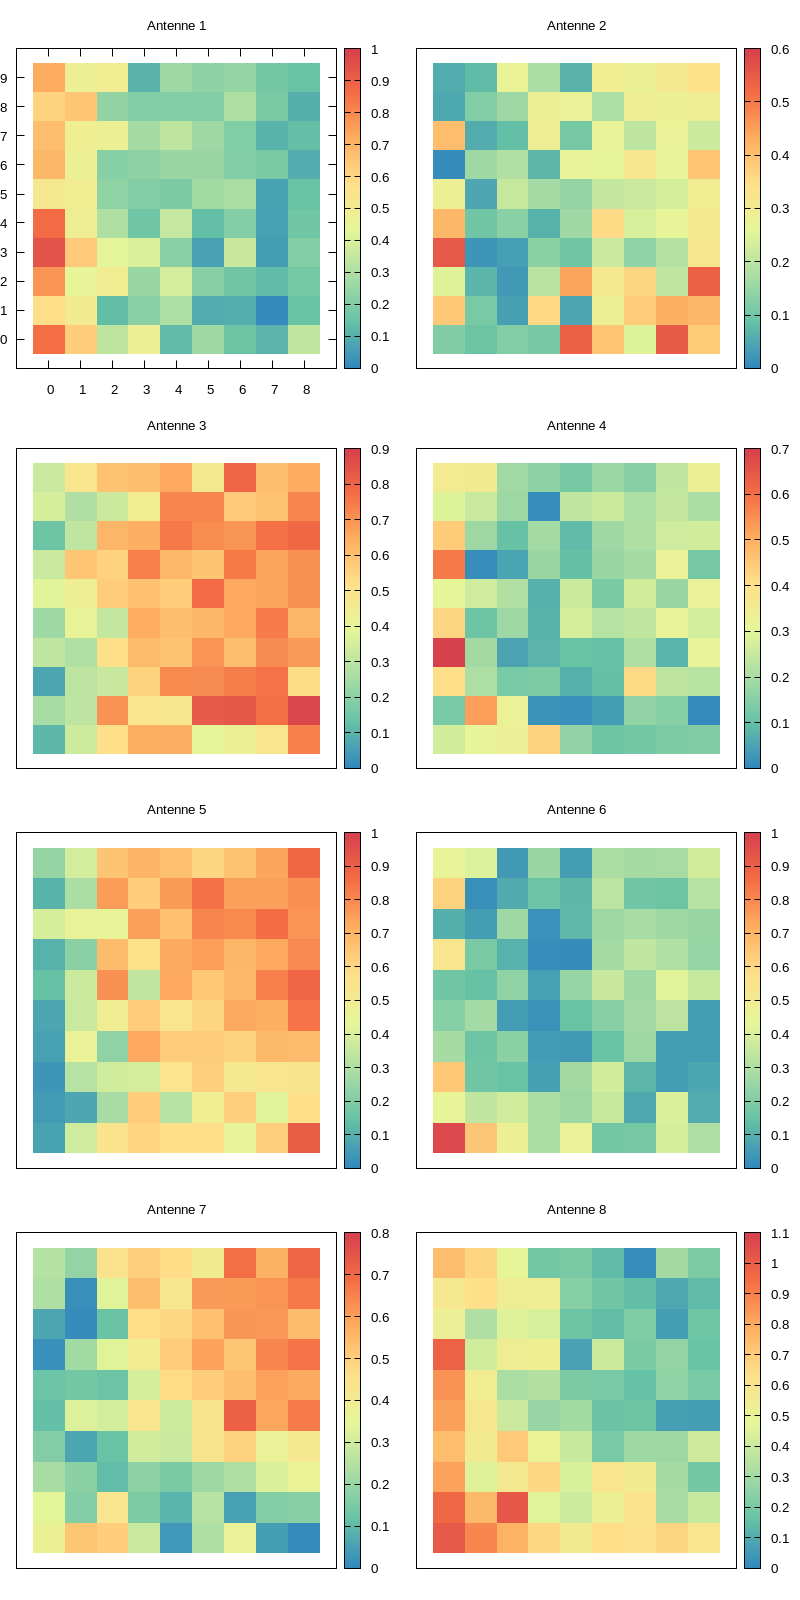
\includegraphics[width=.3\textwidth]{../img/result.png}
%  \qquad
%  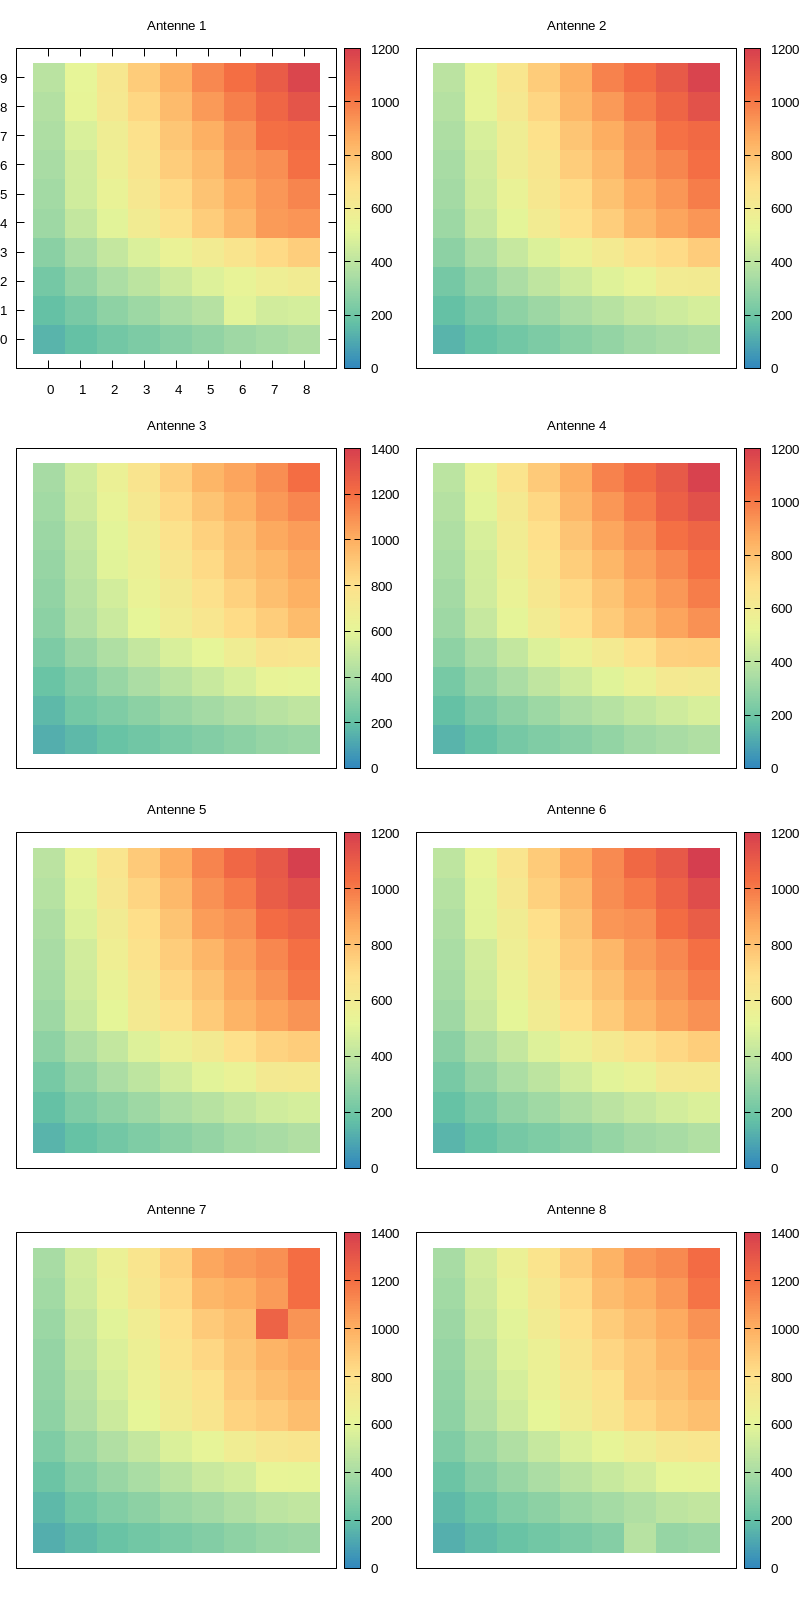
\includegraphics[width=.3\textwidth]{../img/resultstiming.png}
%  \end{center}
%\end{frame}
%------------------------------------------------------
\subsection{Reale Messwerte}
%------------------------------------------------------
\begin{frame}
  \frametitle{Optimierungsverlauf}
  \begin{center}
  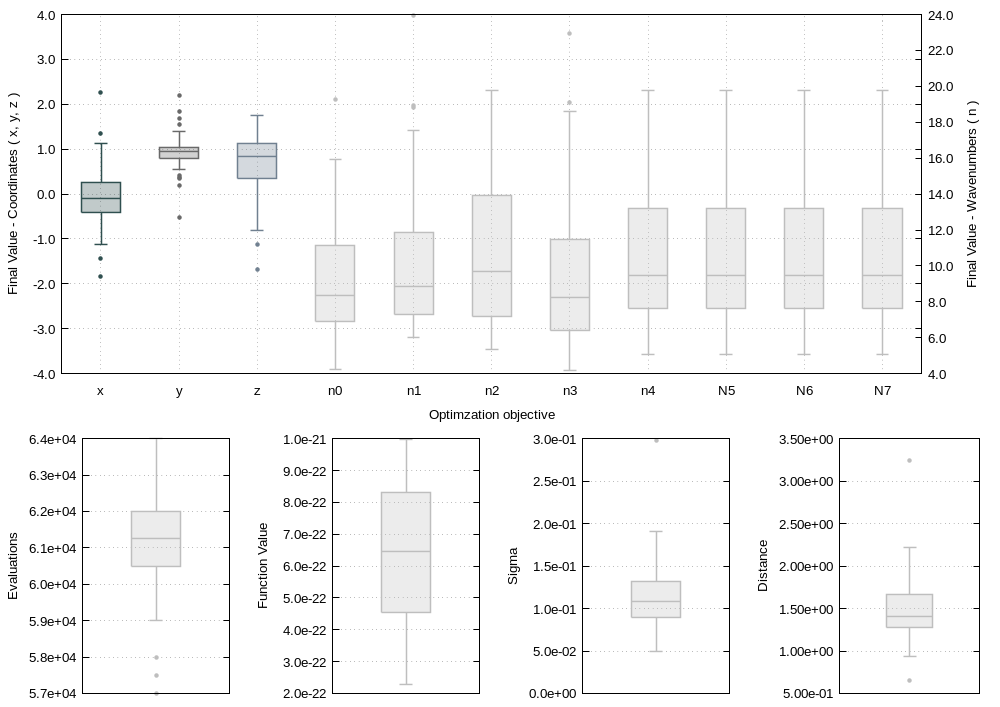
\includegraphics[width=.47\textwidth]{../img/boxes2089.png}
  \qquad
  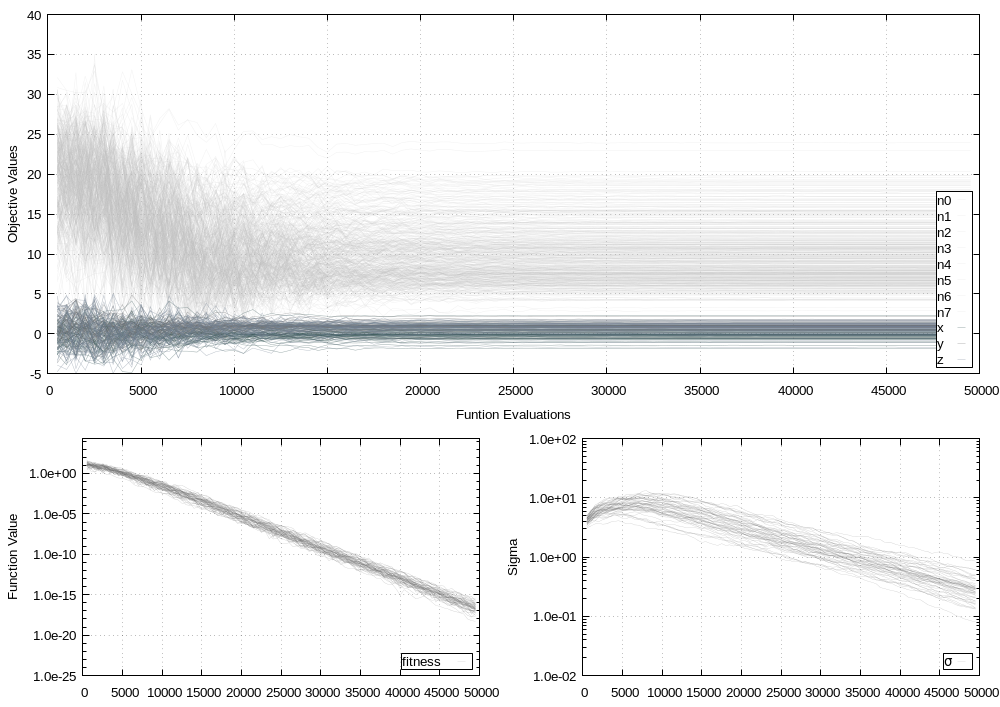
\includegraphics[width=.47\textwidth]{../img/lines2089.png}
  \end{center}
\end{frame}
%------------------------------------------------------
\begin{frame}
  \frametitle{Ergebnisse}
  \begin{center}
  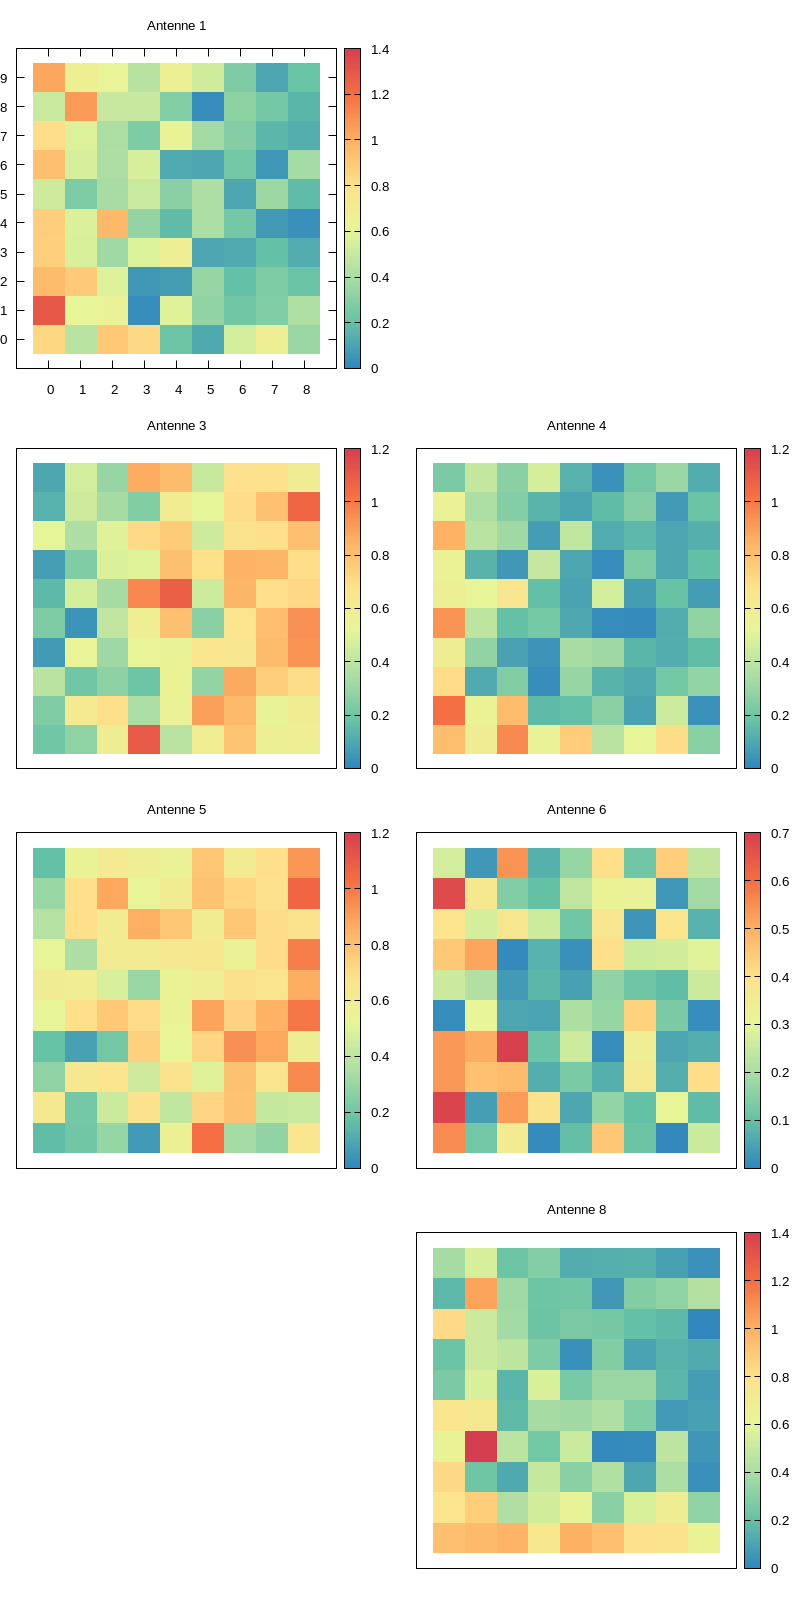
\includegraphics[width=.3\textwidth]{../img/resultRealData.png}
  \qquad
  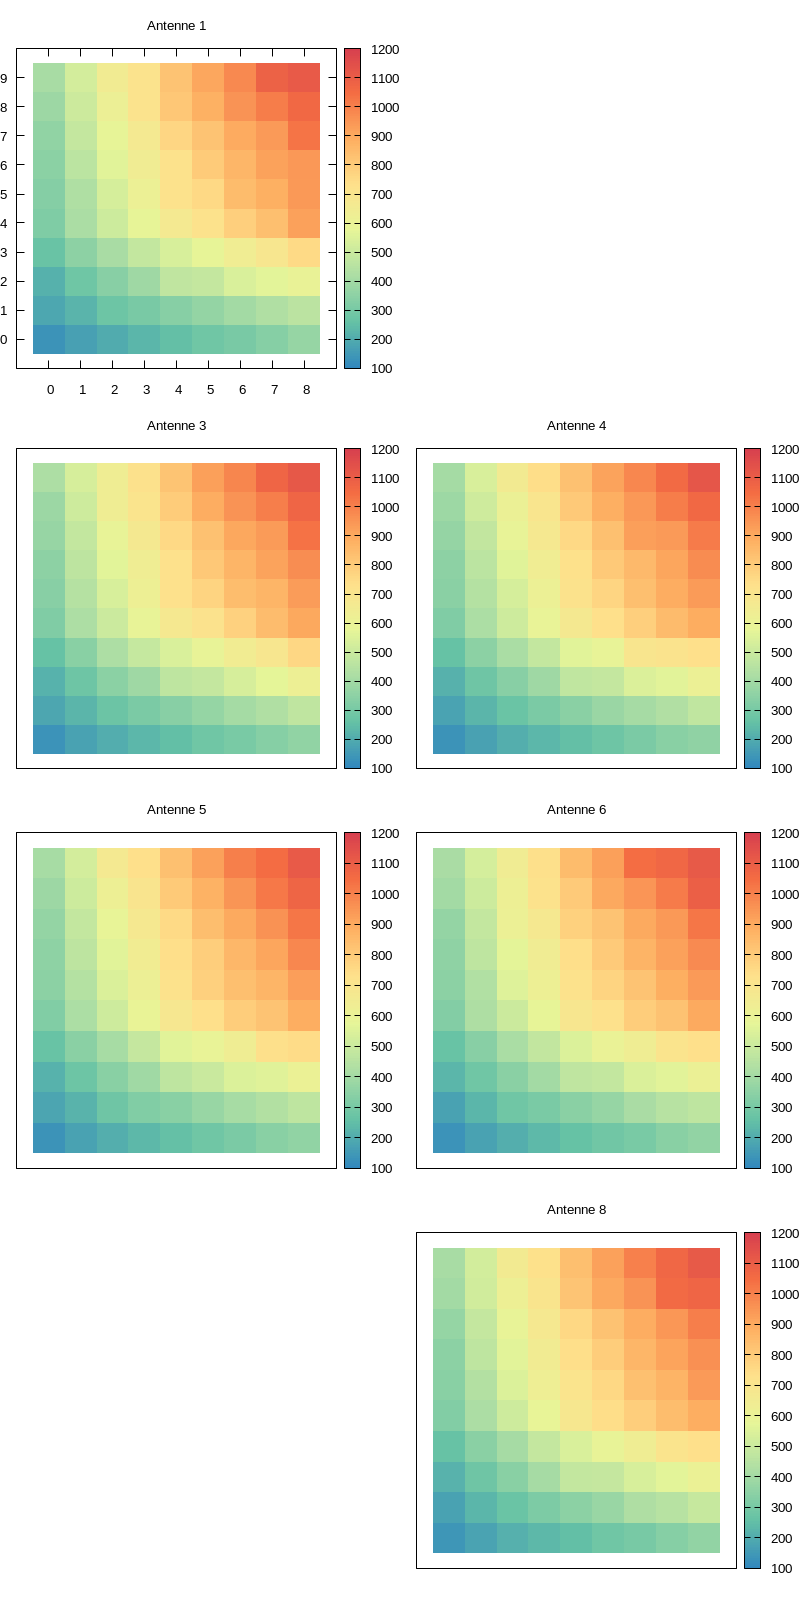
\includegraphics[width=.3\textwidth]{../img/resultstimingreal.png}
  \end{center}
\end{frame}

%------------------------------------------------------
%------------------------------------------------------
\section{Schluss}
%------------------------------------------------------
\begin{frame} %%Eine Folie
  \frametitle{Fazit} %%Folientitel
  \begin{definition} %%Definition
    Fazit hier...
  \end{definition}
\end{frame}
%------------------------------------------------------
\begin{frame}
  	\frametitle{Ende}
  	\centering
	\textbf{Vielen Dank... Zeit für Fragen...}
\end{frame}
%------------------------------------------------------
%------------------------------------------------------
\section*{Appendix}
%
%
%
\begin{appendix}

%----------------------------------------------------------------------------
%----------------------------------------------------------------------------
%\newpage
%
%\begin{center}
%	\huge{Anhänge}
%\end{center}

\normalsize
%
%----------------------------------------------------------------------------
%----------------------------------------------------------------------------
\chapter{Abbildungen}
\section{Messaufbauten}
\begin{figure}[h!]
 \centering
         \includegraphics[width=\textwidth]{img/00_Placeholder.png}
         \caption[PRPS-Kalibiersystem]{PRPS-Messsystem in der "Spinnen"-Konfiguration. Es umfasst vier Messwertgeber und eine Recheneinheit.}
         \label{fig:Spider1}
\end{figure}
\newpage
%
%----------------------------------------------------------------------------
%----------------------------------------------------------------------------
\begin{figure}[h!]
 \centering
         \includegraphics[width=\textwidth]{img/00_Placeholder.png}
         \caption[Übersicht Kalibrieraufbau]{Aufbau des für die Kalibrierung verwendeten Messaufbaus.}
         \label{fig:Spider_setup1}
\end{figure}
\newpage
%
%----------------------------------------------------------------------------
%----------------------------------------------------------------------------
\chapter{Gnuplot Skripte}
\section{Boxplot}
\tiny
\lstinputlisting[
		title=Gnuplot Boxplot-Skript,
		caption=Gnuplot Boxplot-Skript,
		language=Gnuplot,
		numbers=left,
%		frameround=fttt,
		frame=trbl,
		breakatwhitespace=false,         % sets if automatic breaks should only happen at whitespace
   	    breaklines=true,  
		xleftmargin=1cm,
		showstringspaces=false]{../../dev/src/c-cpp/AntConfApp/build/Debug/test/output/mkII/plot/kondensierte_boxen.gp}
\label{append_Script_Box-plot}
\newpage
%
%----------------------------------------------------------------------------
%----------------------------------------------------------------------------
\section{Lineplot}
%\begin{footnote}
\tiny 
%
% listings print source code

% define colors for source code list
\definecolor{colKeys}{rgb}{0,0,1}
\definecolor{colIdentifier}{rgb}{0,0,0}
\definecolor{colComments}{rgb}{0,1,0.3}
\definecolor{colString}{rgb}{0,0.5,0}

\definecolor{dkgreen}{rgb}{0,0.6,0}
\definecolor{gray}{rgb}{0.5,0.5,0.5}

\lstset{language=Matlab,
   keywords={break,case,catch,continue,else,elseif,end,for,function,
   global,if,otherwise,persistent,return,switch,try,while,ones,zeros},
   float=hbp,
   basicstyle=\ttfamily\small,
   identifierstyle=\color{colIdentifier},
   keywordstyle=\color{blue},
   commentstyle=\color{dkgreen},
   stringstyle=\color{red},
   columns=flexible,
   tabsize=2,
   frame=single,
   numbers=left,
   extendedchars=true,
   showspaces=false,
   numberstyle=\tiny\color{gray},
   stepnumber=1,
   numbersep=10pt,
   showspaces=false,
   showstringspaces=false,
   breakautoindent=true}

\lstinputlisting[
		title=Gnuplot Lineplot-Skript,
		caption=Gnuplot Lineplot-Skript,
		language=Gnuplot,
		numbers=left,
%		frameround=fttt,
		frame=trbl,
		breakatwhitespace=false,         % sets if automatic breaks should only happen at whitespace
   	    breaklines=true,  
		xleftmargin=1cm,
		showstringspaces=false]{../../dev/src/c-cpp/AntConfApp/build/Debug/test/output/mkII/plot/kondensierte_linien.gp}
\label{append_Script_Line-plot}
\newpage
%
%----------------------------------------------------------------------------
%----------------------------------------------------------------------------
\section{Scatterplot}
%\begin{footnote}
%
% listings print source code

% define colors for source code list
\definecolor{colKeys}{rgb}{0,0,1}
\definecolor{colIdentifier}{rgb}{0,0,0}
\definecolor{colComments}{rgb}{0,1,0.3}
\definecolor{colString}{rgb}{0,0.5,0}

\definecolor{dkgreen}{rgb}{0,0.6,0}
\definecolor{gray}{rgb}{0.5,0.5,0.5}

\lstset{language=Matlab,
   keywords={break,case,catch,continue,else,elseif,end,for,function,
   global,if,otherwise,persistent,return,switch,try,while,ones,zeros},
   float=hbp,
   basicstyle=\ttfamily\small,
   identifierstyle=\color{colIdentifier},
   keywordstyle=\color{blue},
   commentstyle=\color{dkgreen},
   stringstyle=\color{red},
   columns=flexible,
   tabsize=2,
   frame=single,
   numbers=left,
   extendedchars=true,
   showspaces=false,
   numberstyle=\tiny\color{gray},
   stepnumber=1,
   numbersep=10pt,
   showspaces=false,
   showstringspaces=false,
   breakautoindent=true}

\tiny
\lstinputlisting[
		title=Gnuplot Scatterplot-Skript,
		caption=Gnuplot Scatterplot-Skript,
		language=Gnuplot,
		numbers=left,
%		frameround=fttt,
		frame=trbl,
		breakatwhitespace=false,         % sets if automatic breaks should only happen at whitespace
   	    breaklines=true,  
		xleftmargin=1cm,
		showstringspaces=false]{../../dev/src/c-cpp/AntConfApp/build/Debug/test/output/mkII/plot/scatter.gp}
\label{append_Script_Scatter-plot}
\newpage
%
%----------------------------------------------------------------------------
%----------------------------------------------------------------------------
%\section{Filter Entwurf - Ergebnisse}
%\begin{landscape}
%\label{FirFilterResult}
%\begin{figure} [h]
         \centering
         \caption{ Ergebnisse des Filterentwurfs }
         \label{fig:1}
         \centering
         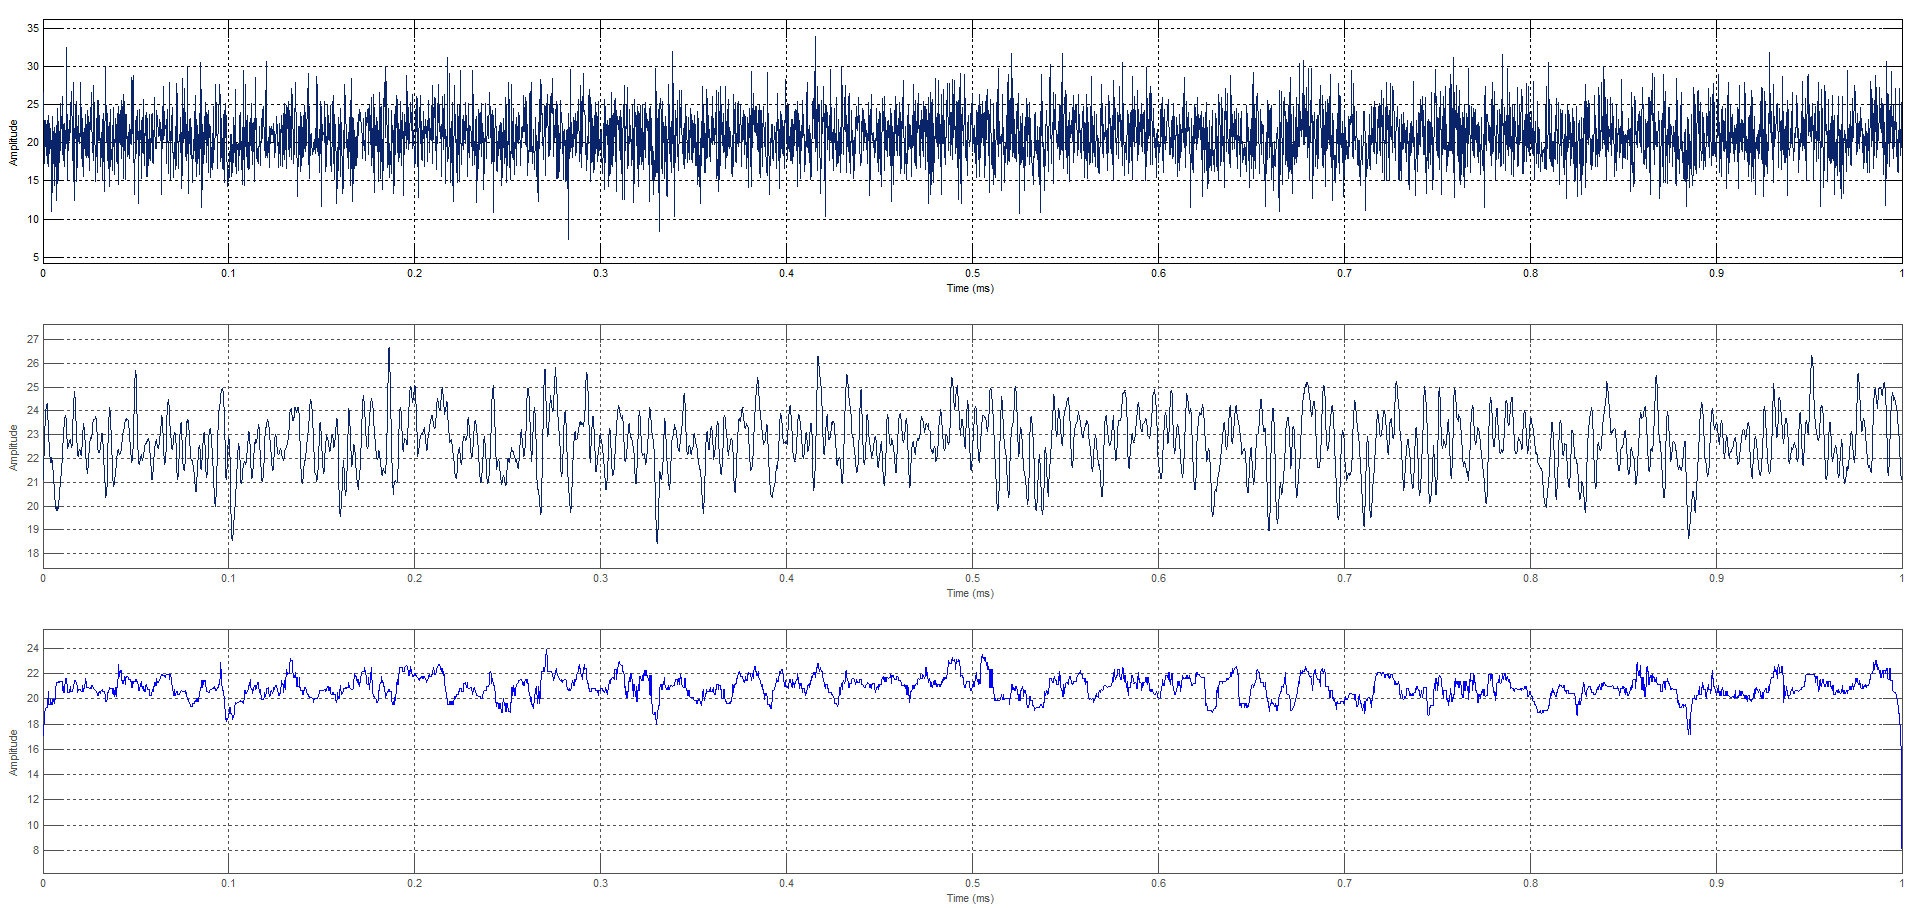
\includegraphics[width=.8\textwidth]{common/img/AmpGefiltert_small.png}\\
\vspace{0.5cm}
Die obere Kurve visualisiert die Rohdaten. Die mittlere Kurve ist das Ergebnis der Tiefpassfilterung für einen der vorgestellten Filter. Die untere Darstellung dient zum Vergleich mit der bisher eingesetzten Filterungsmethode (Median). Es wurden 4096 Messwerte für diese Analyse gesampelt.
\end{figure}
%---------------------------------------------------------------------------------------
\vspace{.5cm}
%---------------------------------------------------------------------------------------
\begin{figure} [h]
         \centering
         \caption{ Spektrum des Messsignals, vor und nach der Filterung  }
         \label{fig:2}
	     \centering
	     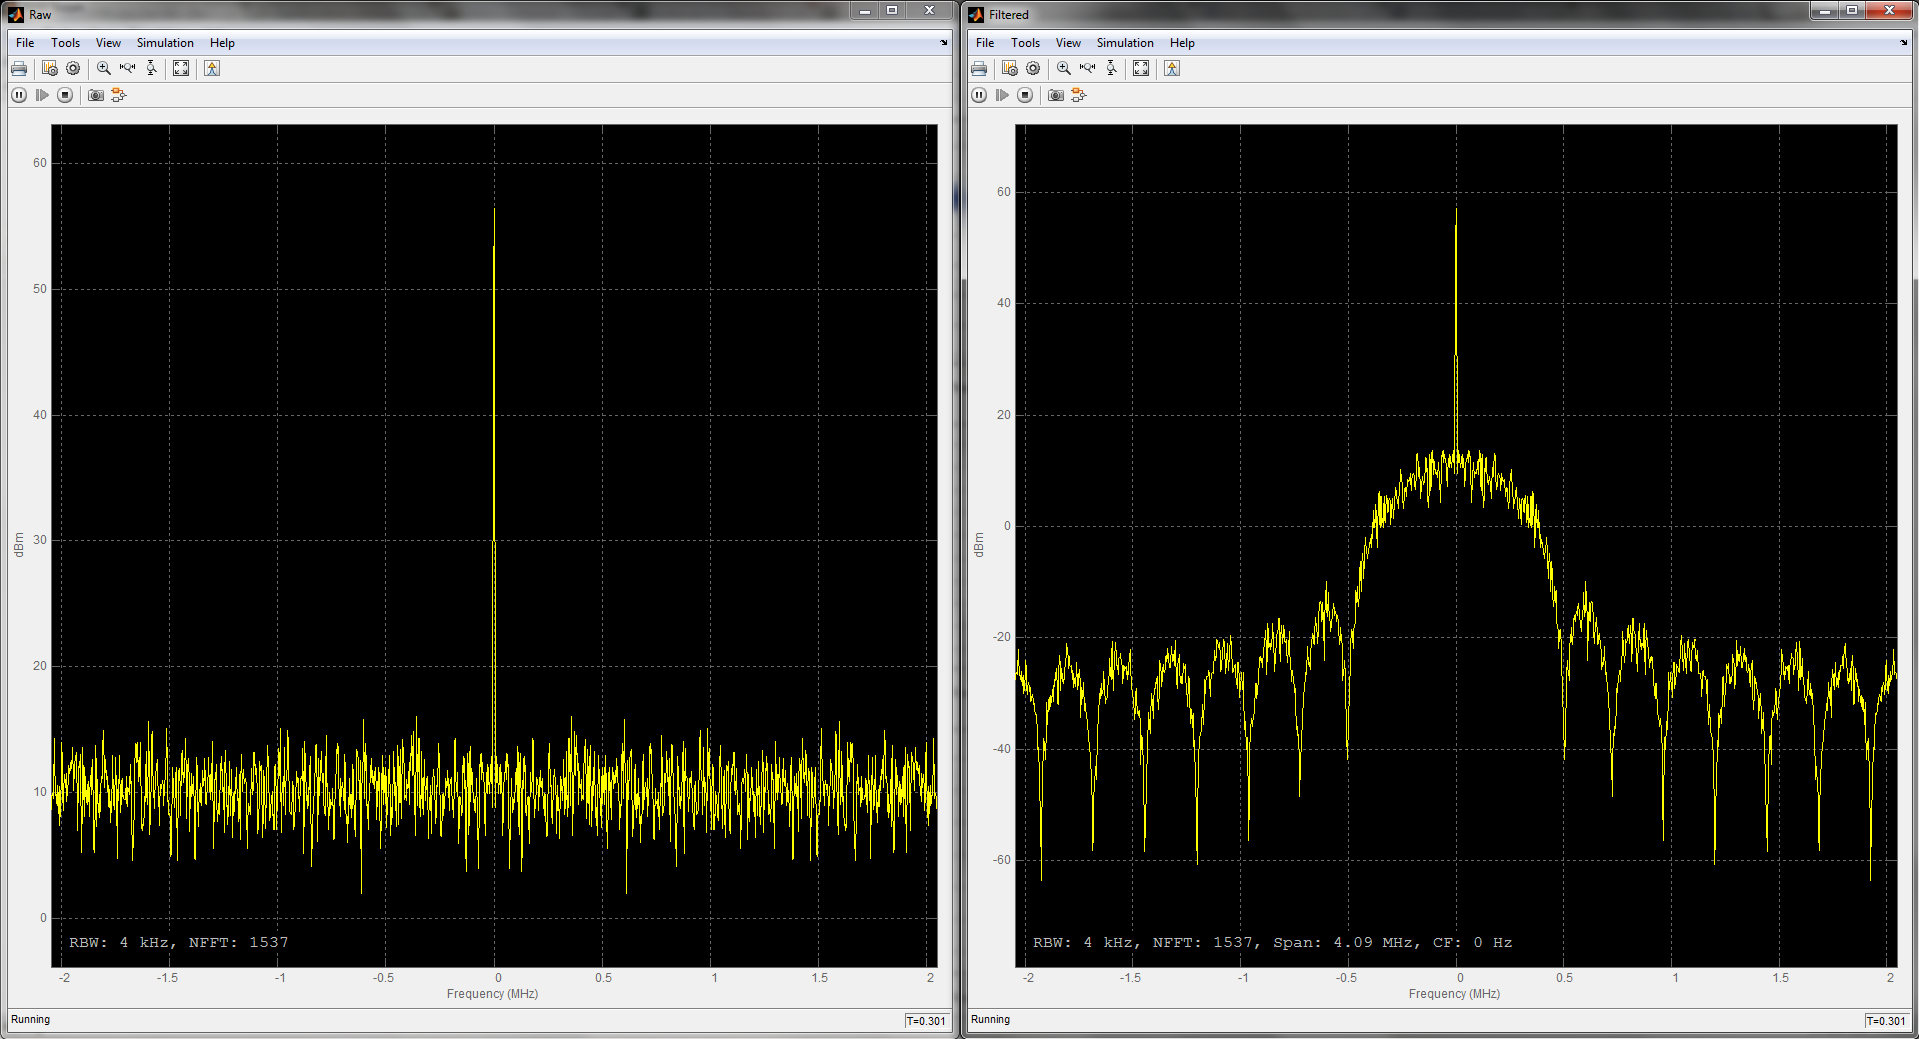
\includegraphics[width=.6\textwidth]{common/img/SpektrumAmp.PNG} \\
\vspace{.2cm}
Die Grafik zeigt das Spektrum des Messsignals der Amplitude. Im linken Bild ist das ungefilterte Signal und im Rechten das gefilterte.
%
\end{figure}
%---------------------------------------------------------------------------------------
\vspace{.5cm}
%---------------------------------------------------------------------------------------
\begin{figure} [h]
         \centering
         \caption{ Frequenzgänge der entworfenen Filter. Beide ähneln sich in den Parametern, verfügen jedoch über etwas unterschiedliche Eckfrequenzen. Als Entwurfsmethode wurde die sog. "Least-squares"-Methode verwendet. Diese Methode liefert gute Ergebnisse im Hinblick auf möglichst kleine Sidelobes und eine geringe Anzahl an Koeffizienten. }
         \label{fig:3}
%         
         \begin{subfigure}[t]{0.5\textwidth}
                 \centering
                 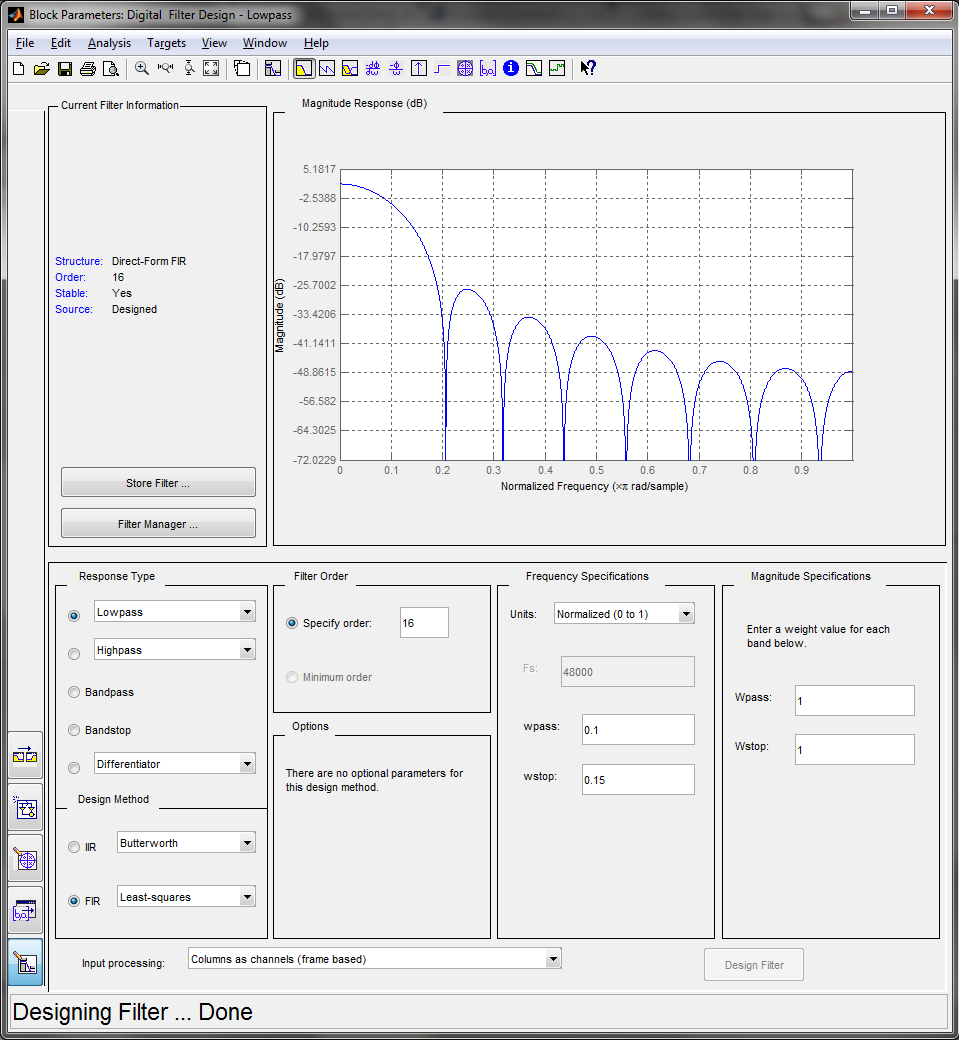
\includegraphics[width=\textwidth]{common/img/filter.png}
                 \vspace{.1cm}
                 \caption{Erstes Filter mit den Parametern wpass~=~0.1 und wstop~=~0.15. Das Ergebnis ist ein schmalbandigeres Filter. }
                 \label{fig:Filter1_A}\textit{}
         \end{subfigure}
%         
\qquad
         \begin{subfigure}[t]{0.5\textwidth}
                 \centering
                 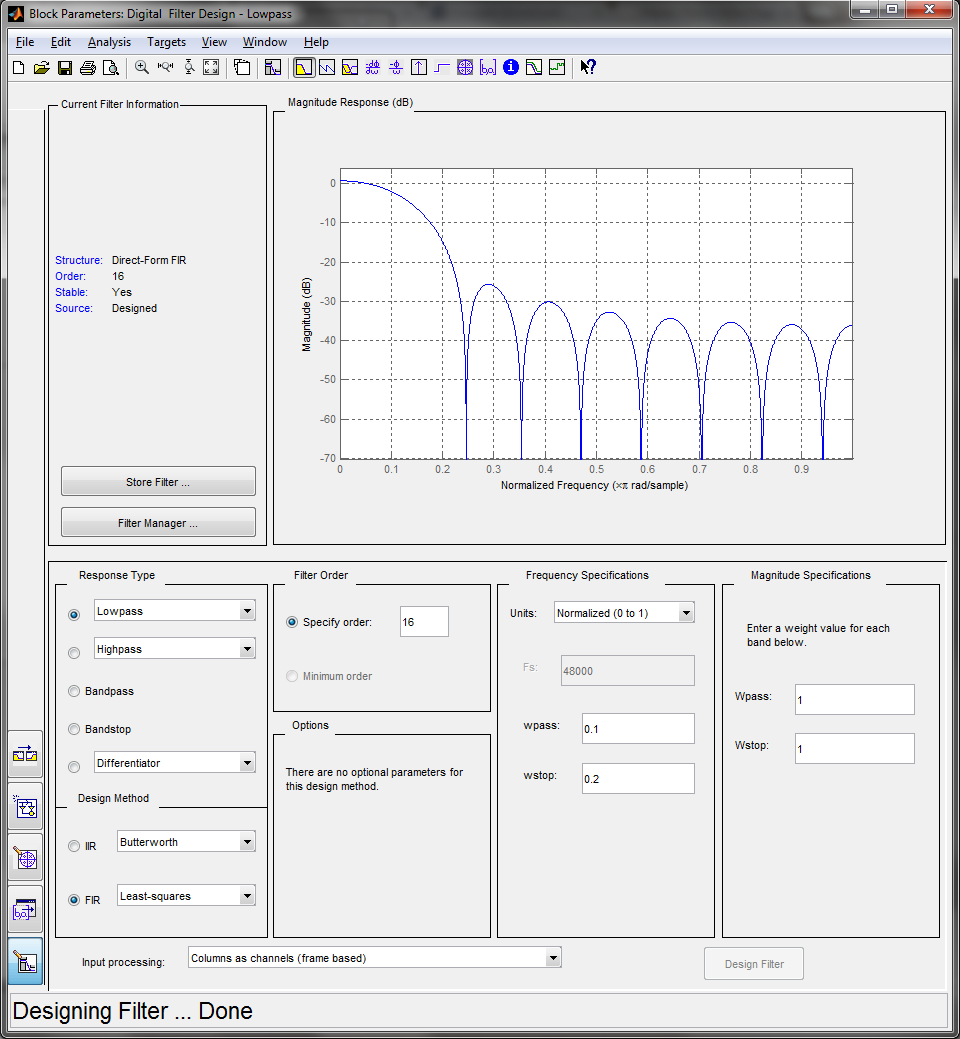
\includegraphics[width=\textwidth]{common/img/filter2.png}
                 \vspace{.1cm}
                 \caption{ Zweites Filter mit den Parametern wpass~=~0.1 und wstop~=~0.2. Der Durchlas bereich ist etwas breiter, dafür sind die Sidelobes stärker gedämpft }
                 \label{fig:Filter2_B}
         \end{subfigure}
%
\end{figure}
%---------------------------------------------------------------------------------------
%\end{landscape}
%
%----------------------------------------------------------------------------
%----------------------------------------------------------------------------
%\newpage
%\begin{landscape}
%	\section{Projektlaufplan KW 31}
%	\label{sec:projectplan}
%	\scalebox{.75}{
%		\begin{ganttchart}[vgrid={draw=none,*1{gray, dashed}},
				hgrid=true,
				today=24,
				title height=1,
				y unit title=0.6cm,
				y unit chart=0.8cm,
				group right shift=0,
				group top shift=.3,
				group height=.3,
				milestone width=.8,
				group peaks={}{}{.2},
				incomplete/.style={fill=black!15}, %
				bar/.style={fill=white}, %
				today label={Heute},
				today rule/.style={dashed, thick}]{44}


\gantttitle{\textbf{2013}}{44} \\
\gantttitlelist{16,...,37}{2} \\
%-------------------------------------------------------------
\ganttgroup{Projekt Evaluation}{3}{14} \\
\ganttbar[progress=100, progress label font=\small\color{black!75},
	progress label anchor/.style={right=4pt}]{Installation der Umgebungen}{3}{6} \\
	
\ganttbar[progress=100, progress label font=\small\color{black!75},
	progress label anchor/.style={right=4pt},
	bar label font=\normalsize\color{black},
	name=rech]{Recherche}{3}{7} \\
	
\ganttmilestone[name=ms1]{Vorstellung der Ergebnisse}{7} \\
	
\ganttbar[progress=90, progress label font=\small\color{black!75},
	progress label anchor/.style={right=4pt},
	bar label font=\normalsize\color{black},
	name=pflichten]
	{Pflichtenheft}{5}{8} \\
	
\ganttmilestone[name=ms2]{Pflichtenheft fertig}{8} \\

\ganttbar[progress=100, progress label font=\small\color{black!75},
	progress label anchor/.style={right=4pt},
	bar label font=\normalsize\color{black},
	name=bNumVerf]
	{Einarbeitung num. Verfahren}{5}{16} \\

\ganttbar[progress=95, progress label font=\small\color{black!75},
	progress label anchor/.style={right=34pt},
	bar label font=\normalsize\color{black},
	name=bCMAES]
	{speziell CMA-ES}{7}{10} \\

\ganttmilestone[name=ms3]{Beurteilung num. Verfahren}{16} \\

\ganttlinkedbar[progress=100, progress label font=\small\color{black!75},
	progress label anchor/.style={right=34pt},
	bar label font=\normalsize\color{black}]
	{Shark Einarbeitung}{17}{18} \\

\ganttlinkedmilestone[name=ms7]{Abschluss Evaluation}{18} \\
	
%-------------------------------------------------------------
\ganttgroup{Erstellung Prototyp}{15}{26} \\
\ganttgroup{(optional)}{15}{18} \\
\ganttbar[progress=25, progress label font=\small\color{black!75},
	progress label anchor/.style={right=4pt},
	bar label font=\normalsize\color{black}]
	{(Entwurf digi. Filter)}{15}{15} \\

\ganttlinkedbar[progress=10, progress label font=\small\color{black!75},
	progress label anchor/.style={right=4pt},
	bar label font=\normalsize\color{black},
	name=bImpFPGA]
	{(Implementation FPGA)}{16}{18} \\

\ganttmilestone[name=ms4]{(Verifikation dig. Filter)}{18} \\
	
\ganttbar[progress=90, progress label font=\small\color{black!75},
	progress label anchor/.style={right=4pt},
	bar label font=\normalsize\color{black},
	name=bImplAlgo]
	{Implementation Algorithmus}{15}{26} \\

\ganttlinkedmilestone[name=ms5]{Implementation Done}{26} \\

%-------------------------------------------------------------
\ganttgroup{Verifikation}{27}{34} \\
\ganttbar[progress=10, progress label font=\small\color{black!75},
	progress label anchor/.style={right=4pt},
	bar label font=\normalsize\color{black},
	name=bVerf]
	{Durchf\"uhrung Verifikation}{27}{34} \\

\ganttlinkedmilestone[name=ms6]{Verifikation Done}{34} \\

%-------------------------------------------------------------
\ganttgroup{Projektdokumentation}{35}{42} \\

\ganttbar[progress=0, progress label font=\small\color{black!75},
	progress label anchor/.style={right=4pt},
	bar label font=\normalsize\color{black},
	name=thesis]
	{Thesis schreiben}{35}{42} \\
	
\ganttmilestone[name=msthesis,milestone label font=\color{red}, 
	milestone/.style={fill=red}]{Abgabe}{42}

%\ganttlink{ms7}{bImplAlgo}
\ganttlink{bImpFPGA}{ms4}
\ganttlink{bNumVerf}{ms3}
\ganttlink{bCMAES}{ms3}
\ganttlink{rech}{ms1}
\ganttlink{pflichten}{ms2}
\ganttlink{thesis}{msthesis}

	\end{ganttchart}
%		}
%\end{landscape}
%
%----------------------------------------------------------------------------

\end{appendix}

%------------------------------------------------------
\bibliographystyle{plaindin}
\bibliography{../../bib/mathesis_collection1}
\end{document}
